%----------------------------------------------------------------------------------------
%	PACKAGES AND OTHER DOCUMENT CONFIGURATIONS
%----------------------------------------------------------------------------------------

\documentclass[10pt, a4paper, twocolumn]{article} % 10pt font size (11 and 12 also possible), A4 paper (letterpaper for US letter) and two column layout (remove for one column)

%%%%%%%%%%%%%%%%%%%%%%%%%%%%%%%%%%%%%%%%%
% Wenneker Article
% Structure Specification File
% Version 1.0 (28/2/17)
%
% This file originates from:
% http://www.LaTeXTemplates.com
%
% Authors:
% Frits Wenneker
% Vel (vel@LaTeXTemplates.com)
%
% License:
% CC BY-NC-SA 3.0 (http://creativecommons.org/licenses/by-nc-sa/3.0/)
%
%%%%%%%%%%%%%%%%%%%%%%%%%%%%%%%%%%%%%%%%%

%----------------------------------------------------------------------------------------
%	PACKAGES AND OTHER DOCUMENT CONFIGURATIONS
%----------------------------------------------------------------------------------------

\usepackage[english]{babel} % English language hyphenation

\usepackage{microtype} % Better typography

\usepackage{amsmath,amsfonts,amsthm} % Math packages for equations

\usepackage[svgnames]{xcolor} % Enabling colors by their 'svgnames'

\usepackage[hang, small, labelfont=bf, up, textfont=it]{caption} % Custom captions under/above tables and figures

\usepackage{booktabs} % Horizontal rules in tables

\usepackage{lastpage} % Used to determine the number of pages in the document (for "Page X of Total")

\usepackage{graphicx} % Required for adding images

\usepackage{enumitem} % Required for customising lists
\setlist{noitemsep} % Remove spacing between bullet/numbered list elements

\usepackage{threeparttable}

\usepackage{sectsty} % Enables custom section titles
\allsectionsfont{\usefont{OT1}{phv}{b}{n}} % Change the font of all section commands (Helvetica)

%----------------------------------------------------------------------------------------
%	MARGINS AND SPACING
%----------------------------------------------------------------------------------------

\usepackage{geometry} % Required for adjusting page dimensions

\geometry{
	top=1cm, % Top margin
	bottom=1.5cm, % Bottom margin
	left=2cm, % Left margin
	right=2cm, % Right margin
	includehead, % Include space for a header
	includefoot, % Include space for a footer
	%showframe, % Uncomment to show how the type block is set on the page
}

\setlength{\columnsep}{7mm} % Column separation width

%----------------------------------------------------------------------------------------
%	FONTS
%----------------------------------------------------------------------------------------

\usepackage[T1]{fontenc} % Output font encoding for international characters
\usepackage[utf8]{inputenc} % Required for inputting international characters

\usepackage{XCharter} % Use the XCharter font

%----------------------------------------------------------------------------------------
%	HEADERS AND FOOTERS
%----------------------------------------------------------------------------------------

\usepackage{fancyhdr} % Needed to define custom headers/footers
\pagestyle{fancy} % Enables the custom headers/footers

\renewcommand{\headrulewidth}{0.0pt} % No header rule
\renewcommand{\footrulewidth}{0.4pt} % Thin footer rule

\renewcommand{\sectionmark}[1]{\markboth{#1}{}} % Removes the section number from the header when \leftmark is used

%\nouppercase\leftmark % Add this to one of the lines below if you want a section title in the header/footer

% Headers
\lhead{} % Left header
\chead{\textit{\thetitle}} % Center header - currently printing the article title
\rhead{} % Right header

% Footers
\lfoot{} % Left footer
\cfoot{} % Center footer
\rfoot{\footnotesize Page \thepage\ of \pageref{LastPage}} % Right footer, "Page 1 of 2"

\fancypagestyle{firstpage}{ % Page style for the first page with the title
	\fancyhf{}
	\renewcommand{\footrulewidth}{0pt} % Suppress footer rule
}

%----------------------------------------------------------------------------------------
%	TITLE SECTION
%----------------------------------------------------------------------------------------

\newcommand{\authorstyle}[1]{{\large\usefont{OT1}{phv}{b}{n}\color{DarkRed}#1}} % Authors style (Helvetica)

\newcommand{\institution}[1]{{\footnotesize\usefont{OT1}{phv}{m}{sl}\color{Black}#1}} % Institutions style (Helvetica)

\usepackage{titling} % Allows custom title configuration

\newcommand{\HorRule}{\color{DarkGoldenrod}\rule{\linewidth}{1pt}} % Defines the gold horizontal rule around the title

\pretitle{
	\vspace{-30pt} % Move the entire title section up
	\HorRule\vspace{10pt} % Horizontal rule before the title
	\fontsize{32}{36}\usefont{OT1}{phv}{b}{n}\selectfont % Helvetica
	\color{DarkRed} % Text colour for the title and author(s)
}

\posttitle{\par\vskip 15pt} % Whitespace under the title

\preauthor{} % Anything that will appear before \author is printed

\postauthor{ % Anything that will appear after \author is printed
	\vspace{10pt} % Space before the rule
	\par\HorRule % Horizontal rule after the title
	\vspace{20pt} % Space after the title section
}

%----------------------------------------------------------------------------------------
%	ABSTRACT
%----------------------------------------------------------------------------------------

\usepackage{lettrine} % Package to accentuate the first letter of the text (lettrine)
\usepackage{fix-cm}	% Fixes the height of the lettrine

\newcommand{\initial}[1]{ % Defines the command and style for the lettrine
	\lettrine[lines=3,findent=4pt,nindent=0pt]{% Lettrine takes up 3 lines, the text to the right of it is indented 4pt and further indenting of lines 2+ is stopped
		\color{DarkGoldenrod}% Lettrine colour
		{#1}% The letter
	}{}%
}

\usepackage{xstring} % Required for string manipulation

\newcommand{\lettrineabstract}[1]{
	\StrLeft{#1}{1}[\firstletter] % Capture the first letter of the abstract for the lettrine
	\initial{\firstletter}\textbf{\StrGobbleLeft{#1}{1}} % Print the abstract with the first letter as a lettrine and the rest in bold
}

%----------------------------------------------------------------------------------------
%	BIBLIOGRAPHY
%----------------------------------------------------------------------------------------

\usepackage[backend=bibtex,style=authoryear,natbib=true]{biblatex} % Use the bibtex backend with the authoryear citation style (which resembles APA)

\addbibresource{biblio.bib} % The filename of the bibliography

\usepackage[autostyle=true]{csquotes} % Required to generate language-dependent quotes in the bibliography


%----------------------------------------------------------------------------------------
%	ALESSANDRO'S ADDITIONS
%----------------------------------------------------------------------------------------

\newcommand{\ie}{\textit{i.e.,} }
\newcommand{\eg}{\textit{e.g.,} }
\newcommand{\wrt}{\textit{w.r.t.\ }}

\newcommand{\todobox}[3]{%
	\colorbox{#1}{\textcolor{white}{\sffamily\bfseries\scriptsize #2}}%
	~\textcolor{blue}{#3} %
	\textcolor{#1}{$\triangleleft$}%
}
\newcommand{\todo}[1]{\todobox{red}{TODO}{#1}}
\newcommand{\feedback}[1]{\todobox{orange}{OK?}{#1}}
\newcommand{\done}[1]{\todobox{blue}{DONE}{#1}}
\newcommand{\rationale}[1]{\todobox{ForestGreen}{RATIONALE}{#1}}

\usepackage{balance}
\usepackage{subcaption} % Specifies the document structure and loads requires packages

%----------------------------------------------------------------------------------------
%	ARTICLE INFORMATION
%----------------------------------------------------------------------------------------

\title{Effective Methods for Capturing Cattle Rustlers} % The article title

\author{
	\authorstyle{John Marston\textsuperscript{1,2,3} and Bonnie MacFarlane\textsuperscript{2,3}} % Authors
	\newline\newline % Space before institutions
	\textsuperscript{1}\institution{Università degli studi di Padova, Padova, Italy}\\ % Institution 1
}

% Example of a one line author/institution relationship
%\author{\newauthor{John Marston} \newinstitution{Universidad Nacional Autónoma de México, Mexico City, Mexico}}

\date{\today} % Add a date here if you would like one to appear underneath the title block, use \today for the current date, leave empty for no date

%----------------------------------------------------------------------------------------

\begin{document}

\maketitle % Print the title

\thispagestyle{firstpage} % Apply the page style for the first page (no headers and footers)

%----------------------------------------------------------------------------------------
%	ABSTRACT
%----------------------------------------------------------------------------------------

\lettrineabstract{WIP}
%----------------------------------------------------------------------------------------
%	ARTICLE CONTENTS
%----------------------------------------------------------------------------------------

\section{Introduction}

IOT (Internet of Things) devices are usually tiny and connected to a large network of alike where they exchange sensible data.
These devices usually have low computational capabilities and exchange sensible data to each other.
It seems reasonable now that we want a computationally efficient and secure way of attestating the integrity of the network.
Remote Attestation allows to interrogate a network and ask for its status in a decentralized way and can be performed by each node of the network.
Collective Remote Attestation adds on top of this the possibility of checking the status of the whole network in a single operation, possibly fast to compute.
SANA (Secure and Scalable Aggregated Network Attestation) wants to provide an attestation protocol for large IOT deployments.
It does so by utilizing a signature scheme called OAS (Optimistic Aggregated Signature) which allows the aggregation of signatures of different devices, making the verification of this aggregated singature constant to the number of compromised devices in the network, instead of constant with the number of all the devices.
In this article we want to focus on the claims SANA made when it was presented, in particular about its security and its weight among the devices.
SANA comes with some estimations about its memory, communication, and computational costs. But the formulas neglect specifying some variables that prove to be decisive to determine these estimations.
We chose to implement the protocol using an ECC algorithm based on Ethereum to handle the signing and verification phases of the protocol, then we analyzed the results to prove the claims that were given in the SANA paper and at last make some considerations about the criticality of this protocol.
%------------------------------------------------

\subsection{Subsection}

Nam ante risus, tempor nec lacus ac, congue pretium dui. Donec a nisl est. Integer accumsan mauris eu ex venenatis mollis. Aliquam sit amet ipsum laoreet, mollis sem sit amet, pellentesque quam. Aenean auctor diam eget erat venenatis laoreet. In ipsum felis, tristique eu efficitur at, maximus ac urna. Aenean pulvinar eu lorem eget suscipit. Aliquam et lorem erat. Nam fringilla ante risus, eget convallis nunc pellentesque non. Donec ipsum nisl, consectetur in magna eu, hendrerit pulvinar orci. Mauris porta convallis neque, non viverra urna pulvinar ac. Cras non condimentum lectus. Aliquam odio leo, aliquet vitae tellus nec, imperdiet lacinia turpis. Nam ac lectus imperdiet, luctus nibh a, feugiat urna.

\begin{itemize}
	\item First item in a list 
	\item Second item in a list 
	\item Third item in a list
\end{itemize}

Nunc egestas quis leo sed efficitur. Donec placerat, dui vel bibendum bibendum, tortor ligula auctor elit, aliquet pulvinar leo ante nec tellus. Praesent at vulputate libero, sit amet elementum magna. Pellentesque sodales odio eu ex interdum molestie. Suspendisse lacinia, augue quis interdum posuere, dolor ipsum euismod turpis, sed viverra nibh velit eget dolor. Curabitur consectetur tempus lacus, sit amet luctus mauris interdum vel. Curabitur vehicula convallis felis, eget mattis justo rhoncus eget. Pellentesque et semper lectus.

\begin{description}
	\item[First] This is the first item
	\item[Last] This is the last item
\end{description}

Donec nec nibh sagittis, finibus mauris quis, laoreet augue. Maecenas aliquam sem nunc, vel semper urna hendrerit nec. Pellentesque habitant morbi tristique senectus et netus et malesuada fames ac turpis egestas. Maecenas pellentesque dolor lacus, sit amet pretium felis vestibulum finibus. Duis tincidunt sapien faucibus nisi vehicula tincidunt. Donec euismod suscipit ligula a tempor. Aenean a nulla sit amet magna ullamcorper condimentum. Fusce eu velit vitae libero varius condimentum at sed dui.

%------------------------------------------------

\subsection{Subsection}

In hac habitasse platea dictumst. Etiam ac tortor fermentum, ultrices libero gravida, blandit metus. Vivamus sed convallis felis. Cras vel tortor sollicitudin, vestibulum nisi at, pretium justo. Curabitur placerat elit nunc, sed luctus ipsum auctor a. Nulla feugiat quam venenatis nulla imperdiet vulputate non faucibus lorem. Curabitur mollis diam non leo ullamcorper lacinia.

Morbi iaculis posuere arcu, ut scelerisque sem. Class aptent taciti sociosqu ad litora torquent per conubia nostra, per inceptos himenaeos. Mauris placerat urna id enim aliquet, non consequat leo imperdiet. Phasellus at nibh ut tortor hendrerit accumsan. Phasellus sollicitudin luctus sapien, feugiat facilisis risus consectetur eleifend. In quis luctus turpis. Nulla sed tellus libero. Pellentesque metus tortor, convallis at tellus quis, accumsan faucibus nulla. Fusce auctor eleifend volutpat. Maecenas vel faucibus enim. Donec venenatis congue congue. Integer sit amet quam ac est aliquam aliquet. Ut commodo justo sit amet convallis scelerisque.

\begin{enumerate}
	\item First numbered item in a list
	\item Second numbered item in a list
	\item Third numbered item in a list
\end{enumerate}

Aliquam elementum nulla at arcu finibus aliquet. Praesent congue ultrices nisl pretium posuere. Nunc vel nulla hendrerit, ultrices justo ut, ultrices sapien. Duis ut arcu at nunc pellentesque consectetur. Vestibulum eget nisl porta, ultricies orci eget, efficitur tellus. Maecenas rhoncus purus vel mauris tincidunt, et euismod nibh viverra. Mauris ultrices tellus quis ante lobortis gravida. Duis vulputate viverra erat, eu sollicitudin dui. Proin a iaculis massa. Nam at turpis in sem malesuada rhoncus. Aenean tempor risus dui, et ultrices nulla rutrum ut. Nam commodo fermentum purus, eget mattis odio fringilla at. Etiam congue et ipsum sed feugiat. Morbi euismod ut purus et tempus. Etiam est ligula, aliquam eget porttitor ut, auctor in risus. Curabitur at urna id dui lobortis pellentesque.

\begin{table}
	\caption{Example table}
	\centering
	\begin{tabular}{llr}
		\toprule
		\multicolumn{2}{c}{Name} \\
		\cmidrule(r){1-2}
		First Name & Last Name & Grade \\
		\midrule
		John & Doe & $7.5$ \\
		Richard & Miles & $5$ \\
		\bottomrule
	\end{tabular}
\end{table}

%------------------------------------------------
 
\section{Premises}

\begin{figure}
	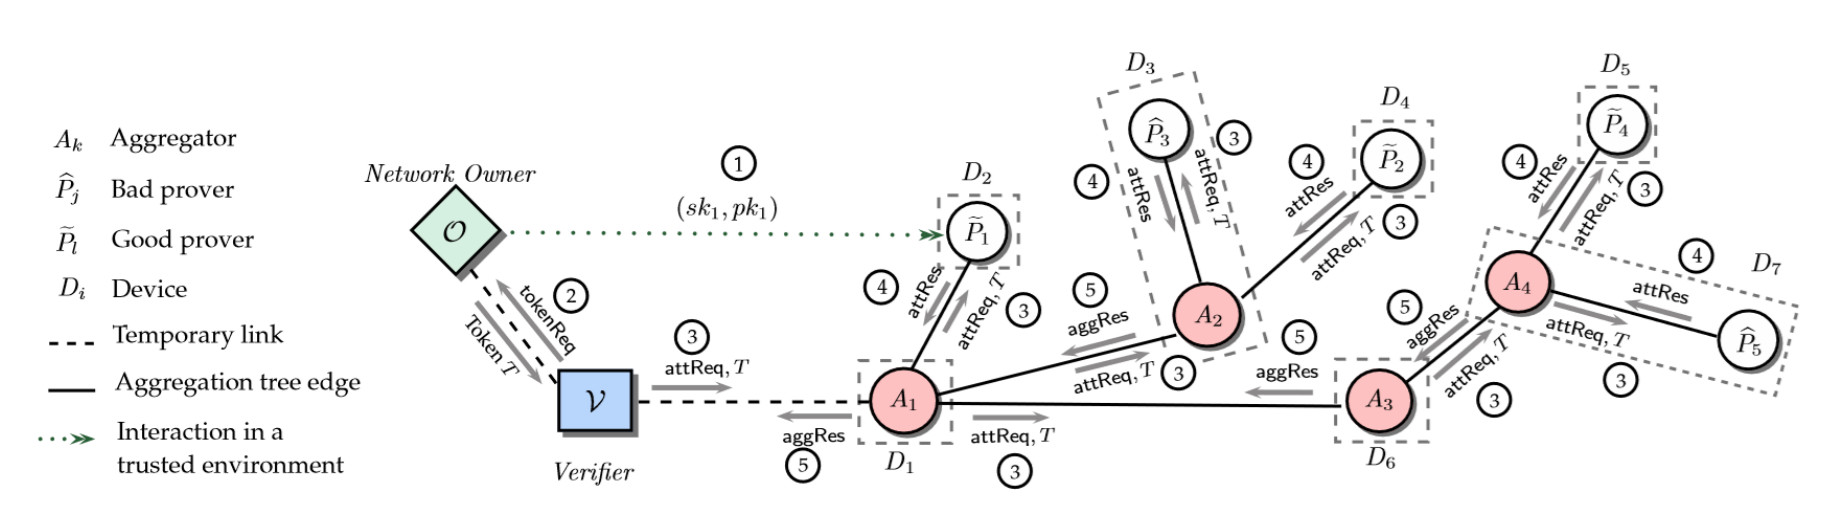
\includegraphics[width=\linewidth]{images/SANA_general.png} % Figure image
	\caption{SANA propagation tree} % Figure caption
	\label{bear} % Label for referencing with \ref{bear}
\end{figure}

Elliptic Curve Cryptography is based, like all Public-key cryptography, on the intractability of some mathematical problems.
For elliptic curve based protocol in particular it's based on the ability to compute easily a point multiplication and the inability to compute the scalar multiplicand given the original point and the result.
All this operations are performed with respect to the finite field the curve is associated with.
In this protocol we use ECC to generate public keys that belong to a multiplicative group that is composed by points on the curve we have chosen for the cryptrographic system.
After that all the signatures are generated by a random oracle as points belonging to the curve. We then use a fancy property of Elliptic curve to perform a bilinear function (called also pairing) on the signature received and a reconstruction of what should be the signature to check if it's authentic in a computationally efficient way.
In SANA the remote attestation process starts from the verifier that sends a request to the Owner that generates a Token and propagates it to the Verifier (containing a challenge that will be proposed to the other nodes in order to certify the authenticity of the attestation request). The Verifier checks the signature and, if it has a positive result, stores the token. \\The Verifier then
the challenge to the closest Aggregator in the propagation tree, this node proceeds to propagate the challenge to its neighbours being other Aggregator
or Provers. The latter then sign a message according to their software configuration being legit or compromised. The signature travel back to the Aggregator
that creates the aggregated signature of its neighbours. Lastly the Verifier checks the aggregated signature of all the tree and determines which devices
can be trusted and which are compromised.\\
For implementing this protocol we chose an elliptic-curve implementation used in Ethereum and called ''bn128'' as it uses a Barreto-Naehrig curve and it's said to offer 128 bits security.


\section{Implementation and analysis}

We wrote an implementation of the algorithm in python, we first defined all the different classes in order to simulate all the nodes (Prover, Aggregator, Owner and Verifier) where neighbours can be assigned to each node in order to resemble a static network configuration.
Before utilizing ''bn128'' we tried to define our curve for the ECC cryptography implementation but for the vast majority of curves that you can choose don't have an easily computable bilinear map, so they were not suitable for our work. At last we decided to use an already existing curve called Barreto-Naherig curve.
After choosing the curve we incorporated the ''bn128'' implementation in our code adding various helping function to generate the keys, software configurations, tokens and challenges.
This implementation uses the Barreto-Naehrig curve on a finite field Zp with p of 256 bits, for the computation of the bilinear map this implementation relies on the Tate-pairing technique which is the fastest for this task. In fact, compared to the Weil pairing the Tate pairing requires only one iteration of the Miller's loop function instead of three simplyfying a lot the computation of the pairing.

We now proceed to evaluate the computational, memory and communication costs of SANA for Provers and Aggregators since we can't make assumption on their costs and the algorithm needs to be feasible even for low-end devices.
Starting from the computational cost we can see that the most complex functions of the protocol are the sign and verify functions as they both have to perform operations on the elliptic curve that require several multiplication to be executed.
\begin{table}
	\caption{Computational cost for each function}
	\centering
	\begin{tabular}{llr}
		\toprule
		Function & Node & Cost \\
		\midrule
		Sign & Prover & $O(n^2log(n))$ \\
		Aggregate & Aggregator & $O(n log(n))$ \\
		Verify & Verifier & $O(n^2log(n))$ \\
		\bottomrule
	\end{tabular}
\end{table}
So we can safely say that the highest cost falls on the provers while the aggregators, which only have to perform one multiplication between objects.

\section{Methods and tools}

For what concerns the work shown above, we wrote our implementation in python and ran it on a google colab instance with multi-threading enabled in order to resemble the possible interaction with the network.
We then executed experiments with different number of provers, different compromised devices rate in order to extract execution time for the most important step of the algorithm.
After that we proceded by performing theorical considerations and calculations in order to estimate the computational complexity, the memory and communication cost, and the total time of the algorithm.
\section{Results}

In hac habitasse platea dictumst. Vivamus eu finibus leo. Donec malesuada dui non sagittis auctor. Aenean condimentum eros metus. Nunc tempus id velit ut tempus. Quisque fermentum, nisl sit amet consectetur ornare, nunc leo luctus leo, vitae mattis odio augue id libero. Mauris quis lectus at ante scelerisque sollicitudin in eu nisi. Nulla elit lacus, ultricies eu erat congue, venenatis semper turpis. Ut nec venenatis velit. Mauris lacinia diam diam, ac egestas neque sodales sed. Curabitur eu diam nulla. Duis nec turpis finibus, commodo diam sed, bibendum erat. Nunc in velit ullamcorper, posuere libero a, mollis mauris. Nulla vehicula quam id tortor ornare blandit. Aenean maximus tempor orci ultrices placerat. Aenean condimentum magna vulputate erat mattis feugiat.

\section{Conclusions}

In hac habitasse platea dictumst. Vivamus eu finibus leo. Donec malesuada dui non sagittis auctor. Aenean condimentum eros metus. Nunc tempus id velit ut tempus. Quisque fermentum, nisl sit amet consectetur ornare, nunc leo luctus leo, vitae mattis odio augue id libero. Mauris quis lectus at ante scelerisque sollicitudin in eu nisi. Nulla elit lacus, ultricies eu erat congue, venenatis semper turpis. Ut nec venenatis velit. Mauris lacinia diam diam, ac egestas neque sodales sed. Curabitur eu diam nulla. Duis nec turpis finibus, commodo diam sed, bibendum erat. Nunc in velit ullamcorper, posuere libero a, mollis mauris. Nulla vehicula quam id tortor ornare blandit. Aenean maximus tempor orci ultrices placerat. Aenean condimentum magna vulputate erat mattis feugiat.

%----------------------------------------------------------------------------------------
%	BIBLIOGRAPHY
%----------------------------------------------------------------------------------------

\printbibliography[title={Bibliography}] % Print the bibliography, section title in curly brackets

%----------------------------------------------------------------------------------------

\end{document}
